\documentclass{beamer}

\usetheme{CambridgeUS}
\usecolortheme{spruce}
\useinnertheme{rectangles}
\usepackage[utf8]{inputenc}
\usepackage[czech]{babel}
\usepackage{graphicx}
\usepackage{amsmath}
\usepackage{color}
\usepackage{listings}
\lstset{
    breaklines=true,
    xleftmargin=\parindent,
    language=C++,
    showstringspaces=false,
    basicstyle=\footnotesize\ttfamily,
    keywordstyle=\color[rgb]{0,0,1},
    commentstyle=\color[rgb]{0.026,0.112,0.095},
    stringstyle=\color[rgb]{0.627,0.126,0.941},
}

\begin{document}
\setbeamertemplate{caption}{\raggedright\insertcaption\par}

\title[ReCodEx -- ReCodEx Code Examiner] % (optional, only for long titles)
{ReCodEx -- ReCodEx Code Examiner}
\author[Buchar, Polanka, Stefan]{J. Buchar, M. Polanka, P. Stefan}
\institute[] % (optional)
{
  Matematicko-fyzikální fakulta\\
  Univerzita Karlova v Praze
}
\date[30. 1. 2018]{} % (optional)
\subject{Computer Science}
%\logo{
\includegraphics[width=0.2\textwidth]{images/logo_recodex.png}}
\titlegraphic{
\includegraphics[width=0.5\textwidth]{images/logo_recodex.png}}

\frame{\titlepage}

\section{ReCodEx}

\begin{frame}
	\frametitle{Motivace}
	\begin{itemize}
		\item Digitalizace výuky (programování na papír)
		\item Ruční kontrola cvičících je zdlouhavá
		\item Specializované vyhodnocovací frameworky
		\item Obecné vyhodnocovací řešení neexistuje
	\end{itemize}
\end{frame}

\begin{frame}
	\frametitle{ReCodEx}
	\begin{itemize}
		\item Systém pro automatické vyhodnocování studentských prací
		\item Učitelé připravují automatizované úlohy
		\item Studenti odevzdávají řešení formou zdrojových kódů programů
		\item Systém řešení zkompiluje a bezpečně vyhodnotí na sadě připravených testů
		\begin{itemize}
			\item Student dostane zpětnou vazbu téměř okamžitě
			\item Učitel vidí odevzdané výsledky a může upravit hodnocení
		\end{itemize}
		\item Jazyky: C, C++ , Pascal, Java, C\#, JS, PHP, Python
		\item V provozu od října 2017
	\end{itemize}
\end{frame}

\begin{frame}
	\frametitle{CodEx vs. ReCodEx}
	\begin{itemize}
		\item Zastaralý frontend CodExu
		\item Sandbox nepodporuje paralelní programy
		\item Omezená vyhodnocovací pipeline (kompilace/spuštění/vyhodnocení)
		\item Pevně svázané komponenty CodExu
		\item Nutnost separátních instancí pro různé programovací jazyky
	\end{itemize}
\end{frame}

\begin{frame}
	\frametitle{Praktická ukázka}
	\begin{center}
		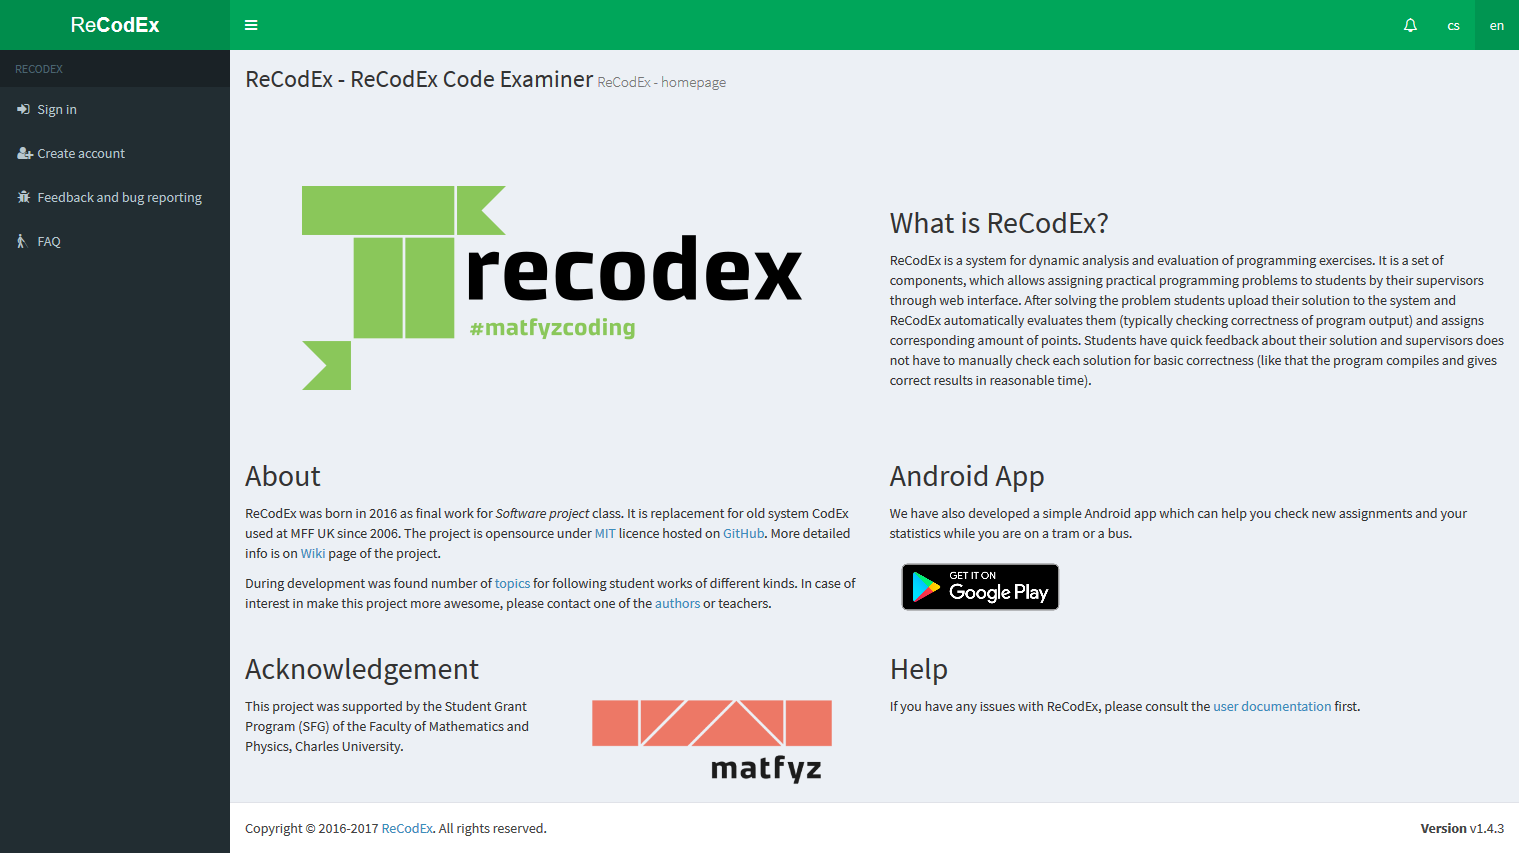
\includegraphics[width=1\textwidth]{images/recodex-screen.png}
	\end{center}
\end{frame}

\begin{frame}
	\frametitle{Úloha "Byrokratický Aparát"}
	\begin{itemize}
		\item Schvalovací proces žádosti na úřadě
		\item Každý úředník má na stole dokument
		\item Dokument přečte, orazítkuje a pošle následujícímu úředníkovi
		\begin{itemize}
			\item Každý úředník má určeno, komu posílá dokumenty
		\end{itemize}
		\item Schvalovací proces končí, když všichni mají na stole dokument, se kterým začínali
		\item Výsledkem je počet kroků k dosažení původního stavu
	\end{itemize}
\end{frame}

\begin{frame}
	\frametitle{Architektura}
	\begin{itemize}
		\item Nezávislé komponenty, které spolu komunikují po síti
		\item Menší aplikace, které se snáze vyvíjejí
		\item Flexibilnější nasazení (přes více strojů)
		\item Webová aplikace je výchozí uživatelské rozhraní pro REST API
		\item REST API 
		\item Backend zajišťuje bezpečné vyhodnocování úloh
		\begin{itemize}
			\item Broker
			\item Worker
			\item Fileserver
			\item Monitor
		\end{itemize}
	\end{itemize}
\end{frame}

\begin{frame}
	\frametitle{Komponenty a komunikace}
	\begin{center}
		\includegraphics[width=1\textwidth]{images/communication.png}
	\end{center}
\end{frame}

\begin{frame}
	\frametitle{HTTP API}
	\begin{itemize}
		\item Uchovává a poskytuje data klientům
		\item Zprostředkovává vyhodnocení úloh
		\item Většina business logiky - uživatelé, skupiny, úlohy, \dots
		\item Podpora alternativních klientů - mobilní aplikace, textové rozhraní, \dots
	\end{itemize}
\end{frame}

\begin{frame}
	\frametitle{Worker}
	\begin{itemize}
		\item Vyhodnocuje studentská řešení v sandboxu
		\item Omezení na čas, paměť, disk, \dots
		\item Izolace (žádný internet, signály, IPC, \dots)
	\end{itemize}
\end{frame}

\begin{frame}
	\frametitle{Broker}
	\begin{itemize}
		\item Spravuje libovolné množství workerů
		\item Rozdělování zátěže
		\item Počítá s výpadky a selháními vyhodnocení
	\end{itemize}
\end{frame}

\begin{frame}
	\frametitle{Scénář -- vyhodnocení úlohy}
	\begin{center}
		\includegraphics[width=1\textwidth]{images/communication.png}
	\end{center}
\end{frame}

\begin{frame}
	\frametitle{Shrnutí}
	\begin{itemize}
		\item Návrh a implementace nového vyhodnocovacího systému
		\item Zapracování požadavků MFF UK
		\item Moderní technologie, rozšiřitelnost, bezpečnost
		\item Automatizované testování
	\end{itemize}
\end{frame}

\section{Závěr}
\begin{frame}
	\frametitle{Závěr}
	\centering
	\LARGE{Děkujeme za pozornost}
\end{frame}

\end{document}
